%% paper preamble
\documentclass[10pt,a4paper, twocolumn]{article}

\usepackage[utf8]{inputenc}
\usepackage[german]{babel}
\usepackage[T1]{fontenc}
\usepackage{fullpage}
\usepackage{graphicx}
\usepackage{listings}
\usepackage{tcolorbox}
\usepackage{url}
\usepackage{float}
\usepackage{nameref}
%\usepackage{subcaption}
\usepackage{hyperref}
\usepackage{xcolor}

\hypersetup{
  colorlinks   = true, 	%Colours links instead of ugly boxes
  urlcolor     = red, 	%Colour for external hyperlinks
  linkcolor    = blue, 	%Colour of internal links
  citecolor   = blue 	%Colour of citations
}
\definecolor{grey}{rgb}{0.9,0.9,0.9}

\setlength{\parindent}{0pt}
\setlength{\columnsep}{0.5cm}

\usepackage[utf8]{inputenc}
\usepackage[german]{babel}
\usepackage[]{csquotes}
\usepackage{amsmath}
\usepackage[]{algorithm2e}

\author{Sven Fiergolla \\ 1252732 \\ s4svfier@uni-trier.de}
\title{Index Construction}



\begin{document}
\maketitle

\section{Einführung}
\paragraph{}
Information Retrieval, zu deutsch Informationsrückgewinnung, ist ein Fachgebiet, welcher sich mit computergestütztem Suchen nach komplexen Inhalten befasst. Der häufigste Anwendungsbereich ist das Suchen von Dokumenten aus einer Sammlung, die für einen Anwender relevant sind. Würde dies auf der unveränderten Datenmenge geschehen, müsste bei jeder Suchanfrage, die komplette Menge an Rohdaten durchsucht werden. Dies ist ein sehr ressourcenintensiver Prozess, daher wird zunächst auf die Hardware sebst eingegangen. Anschließend werden einige Verfahren zum Erstellen eines Index vorgestellt und auf deren Vor- und Nachteile eingegangen.\par

\section{Hardware Constraints}
\begin{figure*}[ht]
  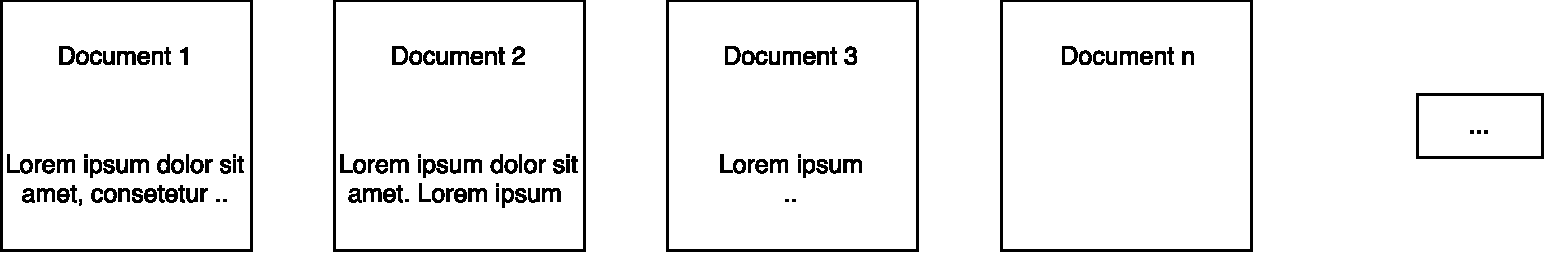
\includegraphics[width=\textwidth]{pdf/Documents.pdf}
  \caption{beispielhafter Dokumenten-Korpus}
  \label{korpus}
\end{figure*}

\paragraph{}
Typische Systemeigenschaften eines Desktop PC im Consumerbereich:
\begin{itemize}
	\item \textit{clock rate} 2-4 GHz, 4-8 Kerne
	\item \textit{main memory} 4-32 Gb
	\item \textit{disk space} $\leq$ 1 TB SSD oder $\geq$ 1 TB HDD
	\begin{itemize}
	\item HDD (hard disk drive)
	\begin{itemize}
	\item \textit{average seek time} zwischen 2 und 10 ms
	\item \textit{transfer} 150 - 300 MB/s
	\end{itemize}
	\item SSD (solid state disk)
	\begin{itemize}
	\item \textit{average seek time} zwischen 0.08 und 0.16 ms
	\item \textit{transfer} Lesen: 545 MB/s, Schreiben: 525 MB/s
	\end{itemize}
	\end{itemize}
\end{itemize}	 
\par

\paragraph{}
Die zu durchsuchende Datensammlung, häufig auch Korpus geannt, befindet sich auf der Festplatte, welche deutlich langsamer arbeitet als der Arbeitsspeicher oder die CPU. Daher stellt die Festplatte in diesem Fall ein Bottleneck\footnote{Wörtlich: \enquote{Flaschenhals} oder \enquote{Engpass}. Gemeint ist ein Engpass beim Transport von Daten, der maßgeblichen Einfluss auf die Arbeitsgeschwindigkeit hat.} dar.
\par

\paragraph{}
Um die intensive Nutzung der Festplatte zu vermeiden, wird eine alterntive Datenstruktur benötigt. Je nach Anforderung kann eine andere Struktur verwendet werden. Für klassisches \enquote{Document Retrival} wird jedoch in der Regel ein so genannter Invertiert Index konstruiert (siehe \nameref{invertedIndex}).
Da mit sich der SSD eine neue Speichertechnologie verbreitet hat, welche deutlich bessere Zugriffszeiten hat als eine HDD, wird diese seperat betrachtet (siehe \nameref{indexSSD}).
\par

\section{Index Construction} \label{IndexConstruction}
\paragraph{}
Um das ressourcenintensive Durchsuchen der Rohdaten zu vermeiden, existieren geeignete Datenstrukturen um Anfragen beantworten zu können, ohne alle Daten durchsuchen zu müssen. Eine einfache geeignete Struktur wäre eine \enquote{Term-Dokument-Matrix}, welche spaltenweise die Dokumente auflistet und zeilenweise das Vorkommen einzelner Worter. Auf einer solchen Matrix lässts sich mit einfachen boolschen Anfragen arbeiten, jedoch hat diese Datenstruktur auch einige Nachteile. Beipsielsweise wächst die Matrix zu stark an für große Sammlungen, es lassen sich keine Komplexeren Anfragen stelle und ein Ranking der Dokumente ist ebenfalls nicht möglich. Daher betrachten wir im Folgenden lediglich den invertierten Index als geeignete Datenstruktur.
\par

\paragraph{}
Um aus einer Sammlung von Rohdaten (Abbildung \ref{korpus}) die relevanten Informationen zu gewinnen, müssen vorher einige Anpassungen getätigt werden. Besteht die Sammlung beispielsweise aus Webseiten, müssen die Informationen vor dem Indizieren aus der \textit{.html}-Datei geparst und von html-Tags befreit werden. In der Regel wird ebenfalls Tokenization und Stemming auf den Text angewendet. Bei der Tokenisierung wird Dokument in kleinste Einheiten (meistens einzene Wörter) geteilt. Stemming erlaubt, dass verschiedene morphologische Varianten eines Wortes auf ihren gemeinsamen Wortstamm zurückgeführt werden (beispielsweise die Deklination von Wortes oder Wörter zu Wort und Konjugation von gesehen oder sah zu seh). Dies ermöglicht, dass bei einer Suchanfrage auch Dokumente gefunden werden können, in denen eine leichte Variation des gesuchten Wortes vorkommt, da beide auf den gleichen Term reduziert werden.
\par

\subsection{Invertierter Index} \label{invertedIndex}
\paragraph{}
Die wesentlichen Schritte zur Erstellung eines invertierten Index sind in Abbildung \ref{postingssList} dargestellt. Zuerst werden alle \enquote{Term-Dokument ID} Paare gesammelt. Diese werden anschließend, dem Term nach, lexikographisch sortiert. Zuletzt werden die Dokument ID's für jeden Term in einer so genannten Postingslist zusammengefasst und Statistiken wie die Frequenz eines Terms berechnet. Die Postingslisten aller Terme bezeichnet man als invertierten Index, da die Zuordnung von Dokumenten auf deren Text invertiert wurde zu der Zuordnung zwischen einem Term und dessen Vorkommen. Bei einer Suchanfrage muss nun lediglich die Postingsliste zu dem gesuchten Term zurückgegeben werden. Aus Performancegründen werden häufig eindeutige Term ID's statt den Termen selbst genutzt. Für kleine Sammlungen kann dies im Arbeitsspeicher geschehen, für größere Sammlungen werden jedoch alternative Verfahren benötigt, auf die im Folgenden eingegangen wird.
\par

\begin{figure*}[ht]
  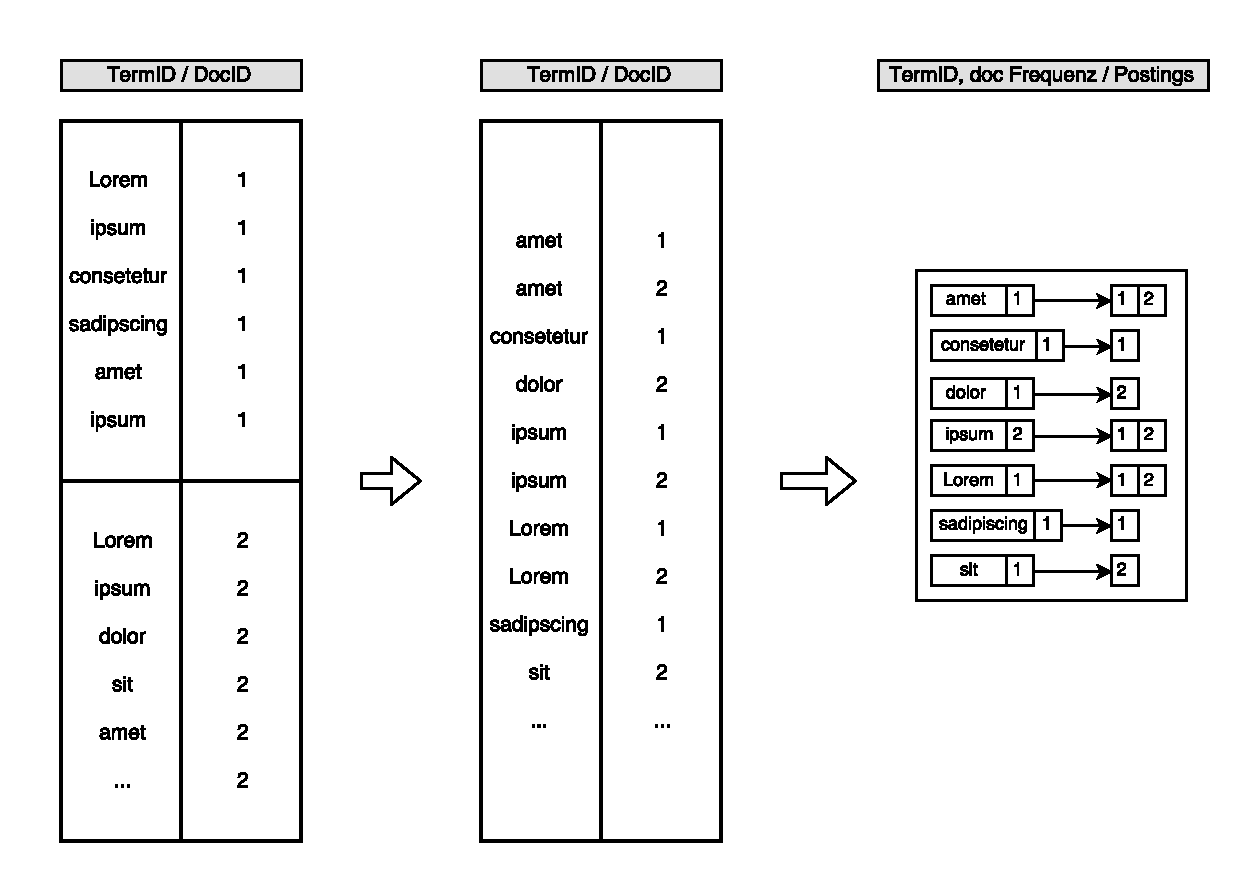
\includegraphics[width=\textwidth]{pdf/postingslist3.pdf}
  \caption{Invertierter Index}
  \label{postingssList}
\end{figure*}

\paragraph{}
In \enquote{Managing Gigabytes: Compressing and Indexing Documents and Images}\cite{ir} wird beispielhaft mit einer Modelsammlung gearbeitet, der Reuters-RCV1. Sie umfasst rund $800.000$ Nachrichtenartikel, ist etwa 1 GB groß und besitzt $100.000.000$ Terme. Die \enquote{Term-Dokument ID} Paare dieser Sammlung auf einer Festplatte zu sortieren ist sehr ineffizient. Beim Sortieren kann von einer Komplexität von $O(n \cdot log_2 (n))$ ausgegangen werden. Möchte man nun alle Terme der Reuters-RCV1 Sammlung sortieren und man von 2 Zugriffen auf die Festplatte beim Sortieren sowie einer durchschnittlichen Zugriffszeit auf die Festplatte von 5ms ausgeht, dauert es in etwa:

\[(100.000.000 \cdot log_2 (100.000.000)) \cdot 2 \cdot (5 \cdot 10^{-3}) \]
\[ = 2.6575424759... \cdot 10^7 \text{ Sekunden}\]
\[ = 307.59 \text{ Tage} \]

Diese Dauer resultiert vorallem aus der hohen Zugriffszeit einer mechanischen Festplatte, da bei jedem wahlfreiem Zugriff der Lesekopf neu positioniert werden muss. Das Lesen von sequenziellen Daten ist deutlich schneller. Ein erster Ansatz ist es, den wahlfreien Zugriff zu minimieren und die Daten hauptsächlich Blockweise zu lesen.
\par

\subsection{Blocked sort-based indexing (BSBI)}

\begin{algorithm}
\caption{BSBI Algorithmus}
 n = 0\;
 \While{all documents have not been processed}{
n = n + 1\;
block = ParseNextBlock()\;
BSBI-INVERT(block)\;
WriteBlockToDisk(block, $f_n$)\;
  }
  MergeBlocks($f_1$, $\cdots$, $f_n$; $f_{merged}$)\;
\end{algorithm}


\begin{figure*}
  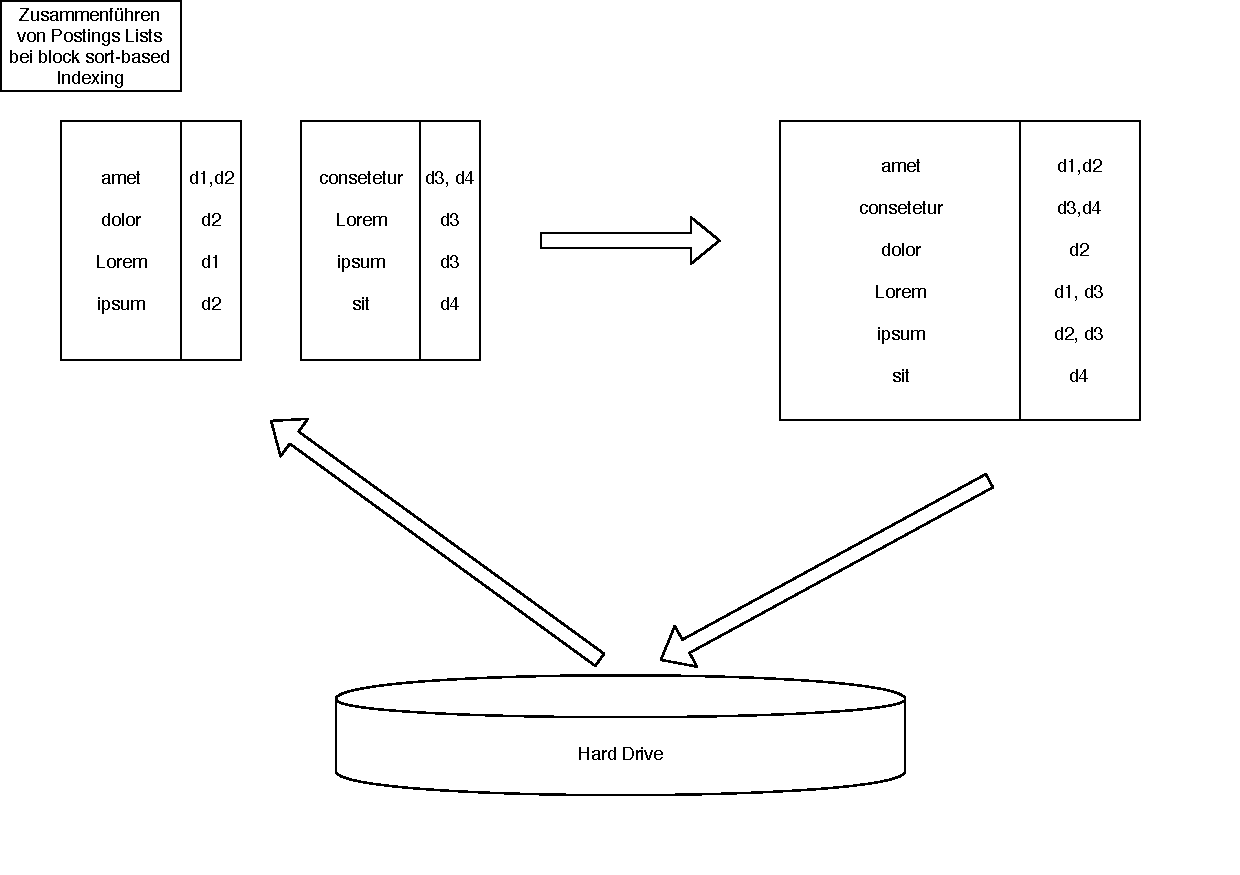
\includegraphics[width=\textwidth]{pdf/BSI_merging.pdf}
  \caption{merging bei BSBI}
\end{figure*}

\subsection{Single-pass in-memory indexing (SPIMI)}

\begin{algorithm}
\caption{SPIMI-invert Algorithmus}
 outputFile = new File()\;
 dictionary = new HashFile()\;
 \While{free memory available}{
 token = next(TokenStream)\;
\eIf{term(token) $\notin$ dictionary}{
PostingsList = AddToDictionary(dictionary, term(token))\;
}{
PostingsList = GetPostingsList(dictionary, term(token))\;
}
\If{full(PostingsList)}{
PostingsList = DoublePostingsList(dictionary, term(token))\;
}
AddToPostingsList(PostingsList, docID(token))\;
SortedTerms = SortTerms(dictionary)\;
WriteBlockToDisk(SortedTerms, dictionary, OutputFile)\;
  }
\end{algorithm}

\subsection{Distributed indexing}
\subsection{Dynamic indexing}
\subsection{andere Indexierungsverfahren}



\section{Indexierung mit Solid State Drives} \label{indexSSD}

\section{Fazit}

\begin{thebibliography}{9}

		\bibitem{ir}
		Christopher D. Manning, Prabhakar Raghavan and Hinrich Schütze \enquote{\href{https://nlp.stanford.edu/IR-book/pdf/04const.pdf}{Introduction to Information Retrieval}}  Cambridge University Press 2008, pp. 1-18 and 67-84.

	 \bibitem{managigGig}
	  Ian H. Witten, Alistair Moffat, Timothy C. Bell \enquote{\href{https://books.google.de/books?id=2F74jyPl48EC&dq=Witten+et+al.+index+1999&lr=&hl=de&source=gbs_navlinks_s}{Managing Gigabytes: Compressing and Indexing Documents and Images}}  Morgan Kaufman Publishers 1999, pp. 223-261.
	
	\bibitem{ssd}
	Yinan Li, Bingsheng He, Robin Jun Yang, Qiong Luo, Ke YiTree (Hong Kong University of Science and Technology) \enquote{\href{http://pages.cs.wisc.edu/~yinan/paper/fdtree_pvldb.pdf}{Indexing on Solid State Drives}} The 36th International Conference on Very Large Data Bases, September 13-17,
2010, Singapore.
\end{thebibliography}
\end{document}